\section{Auswertung}
\label{sec:Auswertung}
\subsection{Bestimmung der Horizontalfeldkomponente des Erdmagnetfelds}
\label{subsec:erdbfeld}
Um die Horizontalkomponente des Erdmagnetfeldes zu bestimmen, werden die zur erzeugung der Felder gemessenen Ströme zunächst mithilfe der Formel
\begin{equation}
  B = \mu_0 I \frac{N}{l}
  \label{eqn:Spulenbfeld}
\end{equation}
in magnetische Feldstärken umgerechnet.
Die dafür benötigten Daten werden der Anleitung\cite{Anleitung} entnommen und lauten:
\begin{table}[H]
  \centering
  \caption{Herstellerangaben für Windungszahl $N$ und Radius $r$ der drei Verwendeten Spulenpaare}
  \label{tab:Spulendaten}
  \begin{tabular}{c|c|c}
    Spule & $N$ &$r$ in cm\\
    \hline
    Horizontalfeld& 151 & 15.79\\
    Vertikalfeld  & 20  & 11.735\\
    RF-Feld       & 11  & 16.39\\
  \end{tabular}
\end{table}
Aus den Angaben für die Vertikalfeldspule ergibt sich ein magnetisches Feld $B_v = \SI{49.19}{\micro\tesla}$
Zur Bestimmung der Horizontalkomponente werden nun die Werte für B-Feld und Frequenz aus Tabelle \ref{tab:messung} je linear gefittet.
\begin{table}
  \centering
  \caption{Werte beider Messungen für horizontales Magnetfeld in Abhängigkeit von der Frequenz für beide Isotope}
  \label{tab:messung}
  \begin{tabular}{|c|c|c||c|c|c|}
    $f_1$ in kHz & $B_{H11}$ in $\mu$T &$B_{H12}$ in $\mu$T&$f_2$ in kHz & $B_{H21}$ in $\mu$T&$B_{H22}$ in $\mu$T\\
    \hline
     98& 21.04 & 21.04& 109& 21.04& 21.04 \\
     194& 21.04& 21.04& 210& 15.78& 15.78\\
     296& 42.09& 42.09& 303& 31.57& 31.57\\
     393& 57.88& 57.88& 400& 52.61& 52.62\\
     499& 78.93& 78.93& 507& 78.93& 78.93\\
     608& 99.97& 99.97& 613& 99.97& 99.97\\
     706& 121.02& 121.02& 707& 99.97& 115.76\\
     802& 99.97& 142.06& 805& 126.28& 163.11\\
     916& 110.50& 194.69& 901& 121.02& 168.38\\
     1016& 121.02& 215.73& 1027& 110.50& 215.73\\
  \end{tabular}
\end{table}
\begin{figure}[H]
  \centering
  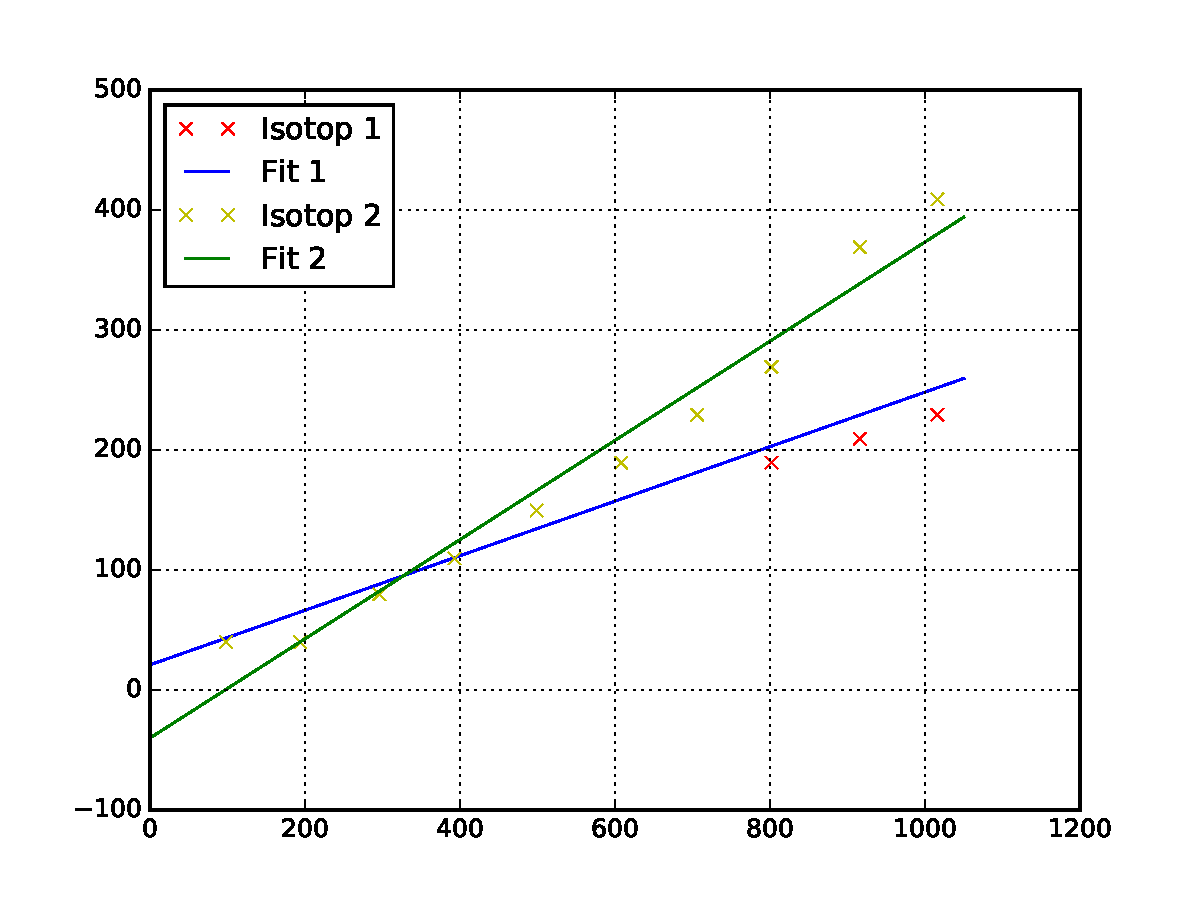
\includegraphics[width=\textwidth]{plots/Bfeldfit1}
  \caption{Lineare Fit der Messwerte der ersten Messung für Frequenz und horizontales Magnetfeld beider Isotope zur Bestimmung der horizontalkomponente des Erdmagnetfeldes.}
  \label{fig:Bfeldfit1}
\end{figure}
\begin{figure}[H]
  \centering
  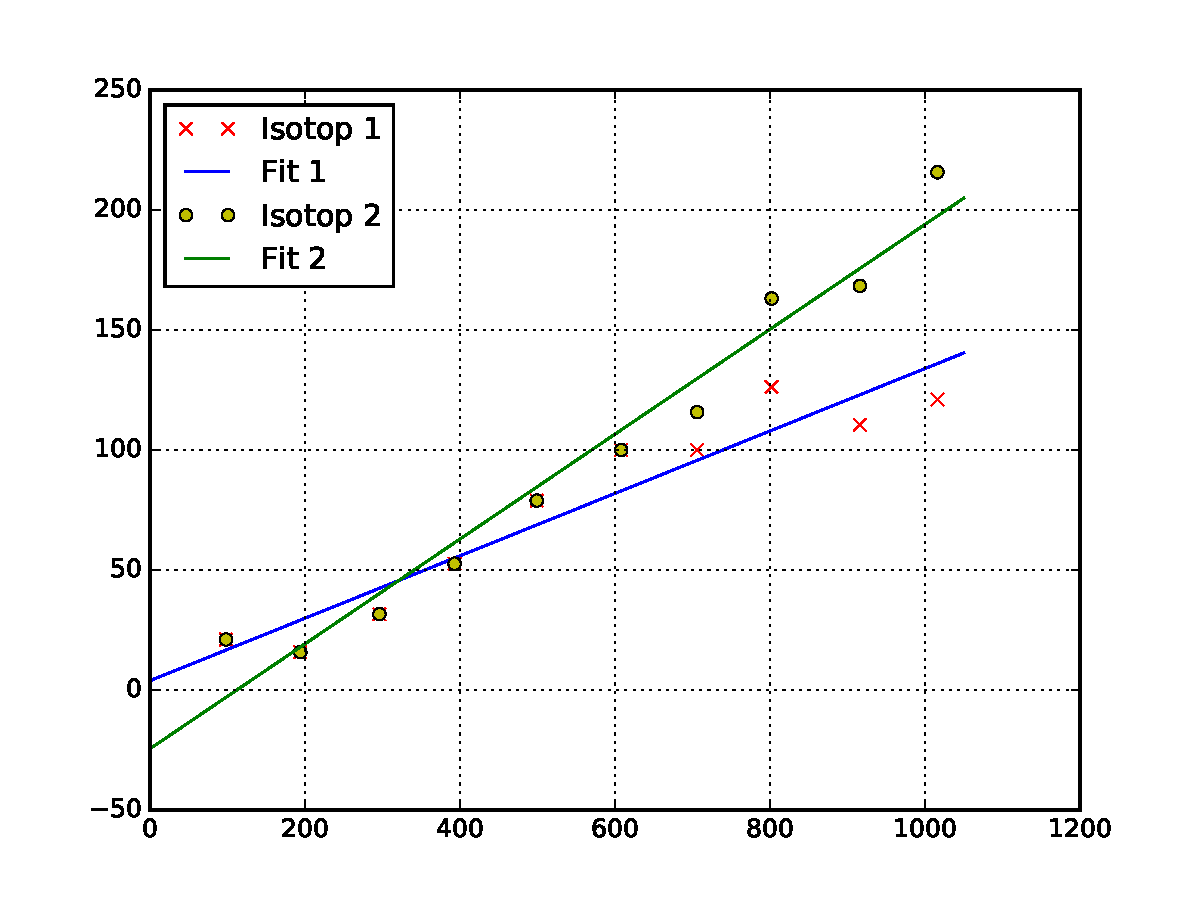
\includegraphics[width=\textwidth]{plots/Bfeldfit2}
  \caption{Lineare Fit der Messwerte der zweiten Messung für Frequenz und horizontales Magnetfeld beider Isotope zur Bestimmung der horizontalkomponente des Erdmagnetfeldes.}
  \label{fig:Bfeldfit2}
\end{figure}
In den Abbildungen \ref{fig:Bfeldfit1} und \ref{fig:Bfeldfit2} sind die Fits beider Messungen zu sehen. Die errechneten Fitparameter lauten:
\begin{center}
  $m_{11} =\SI{0.1199 \pm 0.015}{\micro\tesla\per\kilo\hertz}$ \,\,$b_{11} =\SI{11.06 \pm 9.10}{\micro\tesla}$\\
  $m_{12}=\SI{0.2112 \pm 0.0145}{\micro\tesla\per\kilo\hertz}$ \,\,$b_{11} =\SI{-21.12 \pm 9.08}{\micro\tesla}$\\
  $m_{21} =\SI{0.1300 \pm 0.0144}{\micro\tesla\per\kilo\hertz}$ \,\,$b_{21} =\SI{3.88 \pm 9.03}{\micro\tesla}$\\
  $m_{22}=\SI{2.1847 \pm 0.015}{\micro\tesla\per\kilo\hertz}$ \,\,$b_{22} =\SI{-24.48 \pm 9.44}{\micro\tesla}$\\
\end{center}
Die y-Achsenabschnitte $b_{ij}$ der Ausgleichsrechnungen stehen hierbei für die Horizontalkomponente des Erdmagnetfelds.
\subsection{Berechnung der Landé-Faktoren und der Kernspins}
\label{subsec:lande}
Um die Landé-Faktoren auszurechnen, wird Formel \eqref{eqn:U} aus der Theorie verwendet. In diese Formel wird nun für die Energiedifferenz die Energie der Lichtquanten eingesetzt, die mithilfe der RF-Spule erzeugt werden. Mit der Energie der Photonen $U = h\cdot f$, wobei f die Frequenz und h die Planckkonstante sind, lässt sich die Formel \eqref{eqn:U} jetzt zu
\begin{equation}
  g_F = \frac{h\cdot f}{\mu_B\cdot B}
  \label{eqn:landefaktor}
\end{equation}
umstellen. In diese Gleichung wird nun Steigung $m = \frac{B}{f}$ des Fits aus \ref{subsec:erdbfeld} eingesetzt wodurch sich die Landé-Faktoren zu
\begin{center}
  $g_{F1} = 0.6 \pm 0.07$\\ $g_{F2} = 0.328 \pm 0.022$\\ $g_{F3} = 0.55 \pm 0.06$\\ $g_{F4} =0.327 \pm 0.023$\\
\end{center}
ergeben.\\
Für die Berechnung der Kernspins der beiden Rubidium Isotope wird die Formel \eqref{eqn:gf} nach I umgestellt. Der Elektronenhüllenspin $\text{J} = \frac{1}{2}$ eines Alkaliatoms lässt sich aus der Summe der Spinquantenzahl $\text{S} = \frac{1}{2}$c und der Drehimpulsquantenzahl $\text{L} = 0$ berechnen, woraus $g_J = 2.0023$ folgt. Die Formel \eqref{eqn:gj} verändert sich dann zu
\begin{equation}
  \text{I} = \frac{\frac{g_J}{g_F}-1}{2}
  \label{eqn:kernspin}
\end{equation}.
Die Kernspins, die sich aus den beiden Messungen ergeben lauten dann:
\begin{center}
  $\symup{I_1} = 1.18 \pm 0.20$\\ $\symup{I_2} = 2.56 \pm 0.20$\\ $\symup{I_3} = 1.32 \pm 0.20$\\ $\symup{I_4} = 2.56 \pm 0.21$\\
\end{center}
\subsection{Bestimmung des Isotopenverhältnisses anhand des Ausdrucks}
\label{subsec:iso}
\begin{figure}[H]
  \centering
  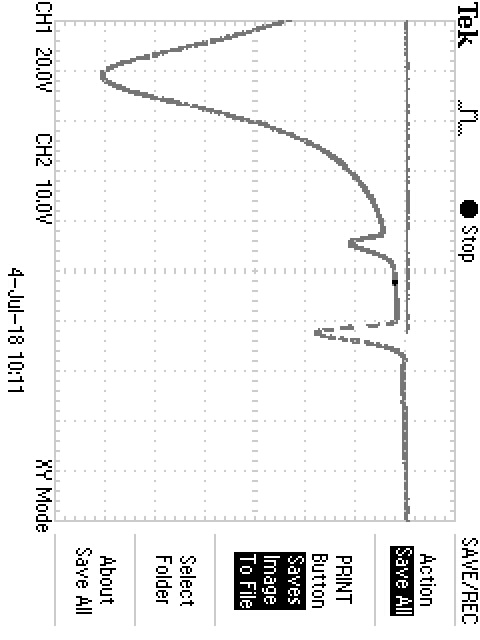
\includegraphics[angle = 90]{TEK0022.JPG}
  \caption{Ausdruck der Transparenzkurve}
  \label{fig:Ausdruck}
\end{figure}
\begin{table}
  \centering
  \caption{Messdaten aus der Vermessung der Minima und daraus berechnete Anteile.}
  \label{tab:Anteil}
  \begin{tabular}{c|c|c}
    &$^{87}\symup{Rb}$ & $^{85}\symup{Rb}$\\
    \hline
    Tiefe in cm& 1.35& 2.1\\
    Anteil in \%&38.84&60.86\\
    Literaturwert:&27.83&72.17\\
    Abweichung in \%&39.56&15.67\\
  \end{tabular}
\end{table}
Aus dem Ausdruck in Abbildung \ref{fig:Ausdruck} wird die Tiefe der beiden Minima in der Transparenz abgelesen. Da sie proportional zur Menge der Isotope in der Probe ist, kann daraus der Anteil der beiden Isotope in der Probe bestimmt werden. Die ermittelten Werte sind in Tabelle \ref{tab:Anteil} aufgelistet.
